\documentclass[conference]{IEEEtran}
\IEEEoverridecommandlockouts
% The preceding line is only needed to identify funding in the first footnote. If that is unneeded, please comment it out.
\usepackage{cite}
\usepackage{amsmath,amssymb,amsfonts}
\usepackage{algorithmic}
\usepackage{graphicx}
\usepackage{textcomp}
\usepackage{xcolor}
\def\BibTeX{{\rm B\kern-.05em{\sc i\kern-.025em b}\kern-.08em
    T\kern-.1667em\lower.7ex\hbox{E}\kern-.125emX}}
\begin{document}

\title{\textbf{Computer Vision Pipeline}
	\\Technical Report}

% Authoren	
\author{

	\IEEEauthorblockN{André Kestler}
	\IEEEauthorblockA{
		\textit{a.kestler@oth-aw.de}\\
	}
	\\
	
	\IEEEauthorblockN{Antonio Vidos}
	\IEEEauthorblockA{
		\textit{a.vidos@oth-aw.de}\\
	}
	\and
	
	\IEEEauthorblockN{Marcus Haberl}
	\IEEEauthorblockA{
		\textit{m.haberl@oth-aw.de}\\
	}
	\\
	
	\IEEEauthorblockN{Tobias Dobmeier}
	\IEEEauthorblockA{
		\textit{t.dobmeier@oth-aw.de}\\
	}
	\and
	
	\IEEEauthorblockN{Tobias Lettner}
	\IEEEauthorblockA{
		\textit{t.lettner@oth-aw.de}\\
	}
	\\
	
	\IEEEauthorblockN{Tobias Weiß}
	\IEEEauthorblockA{
		\textit{t.weiss@oth-aw.de}\\
	}
}


\maketitle

%Hier werden alle Teilabschnitte strukturiert und eingebunden

\begin{abstract}
	Dieser technische Bericht präsentiert die Softwarearchitektur des Projekts ''Computer Vision Pipeline''. Das Hauptziel der Implementierung besteht darin, dem Benutzer die Funktionen gängiger Bildverarbeitungsbibliotheken über eine benutzerfreundliche Anwendung mithilfe einer Cloud-Infrastruktur zugänglich zu machen. 
\end{abstract}


\section{Einführung und Ziele}
\section{Einführung und Ziele}
Hier steht die Einführung und Ziele.

\section{Architektur Allgemein}
\section{Architektur Allgemein}
Hier steht allgemeine Architektur.

\section{Frontend: Benutzerschnittstelle}
\subsection{Frontend: Benutzerschnittstelle}
Das in React geschriebene Frontend besteht aus einer Hauptkomponente, welche aus mehreren Kindkomponenten besteht (siehe Abbildung \ref{fig:frontend}).
Ein \textit{Header}, welcher die Möglichkeit bietet die Seite neuzuladen, Informationen über die Internetseite einzuholen und den Darkmode zu aktivieren, befindet sich am oberen Bildschirmrand.
Über ein Benutzersymbol, werden nach einer Autorisierung weitere Funktionalitäten für Entwickler freigeschalten.
Eine weitere Komponente im oberen Bereich ermöglicht dem Benutzer den Upload eines eigenen oder eines Beispielbildes.
Zwei weitere Komponenten am linken Bildschirmrand, \textit{Selected Image} und \textit{Imagedetails}, sind dafür zuständig das hochgeladene Bild anzuzeigen, sowie die Bildinformationen in Form eines Histogrammes anzuzeigen.
Die Komponente \textit{Availible steps} am rechten Bildschirmrand stellt dem Benutzer alle möglichen Bildoperationen zur Verfügung.
Möchte dieser eine Bildoperation anwenden, muss eine Karte aus der Komponente per Drag and Drop in die dafür vorgesehene Komponente \textit{Pipeline} im Zentrum gezogen werden.
Möchte der Benutzer die Verarbeitung starten, kann dieser das durch das Klicken der Schaltfläche \textit{Start Pipeline} erreichen.
Das Frontend schickt daraufhin alle benötigten Informationen an das Backend.
Das Klicken des Symbols \textit{i} bei einem Verarbeitungsschritt liefert dem Benutzer Informationen zu der jeweiligen Bildoperation.
Hat der Benutzer einen Verarbeitungsschritt abgelegt, kann er über das Klicken des nach unten gerichteten Pfeils die Parameter der Bildoperation konfigurieren.
Klickt der Benutzer auf das Sichbarkeitssymbol eines Verarbeitungsschritts, wird das Zwischenergebnis angezeigt.
Dies ermöglicht es dem Benutzer, Schritt für Schritt Ergebnisse aus den einzelnen Verarbeitungsschritten nachzuvollziehen.
\begin{figure*}[ht]
    \centering
    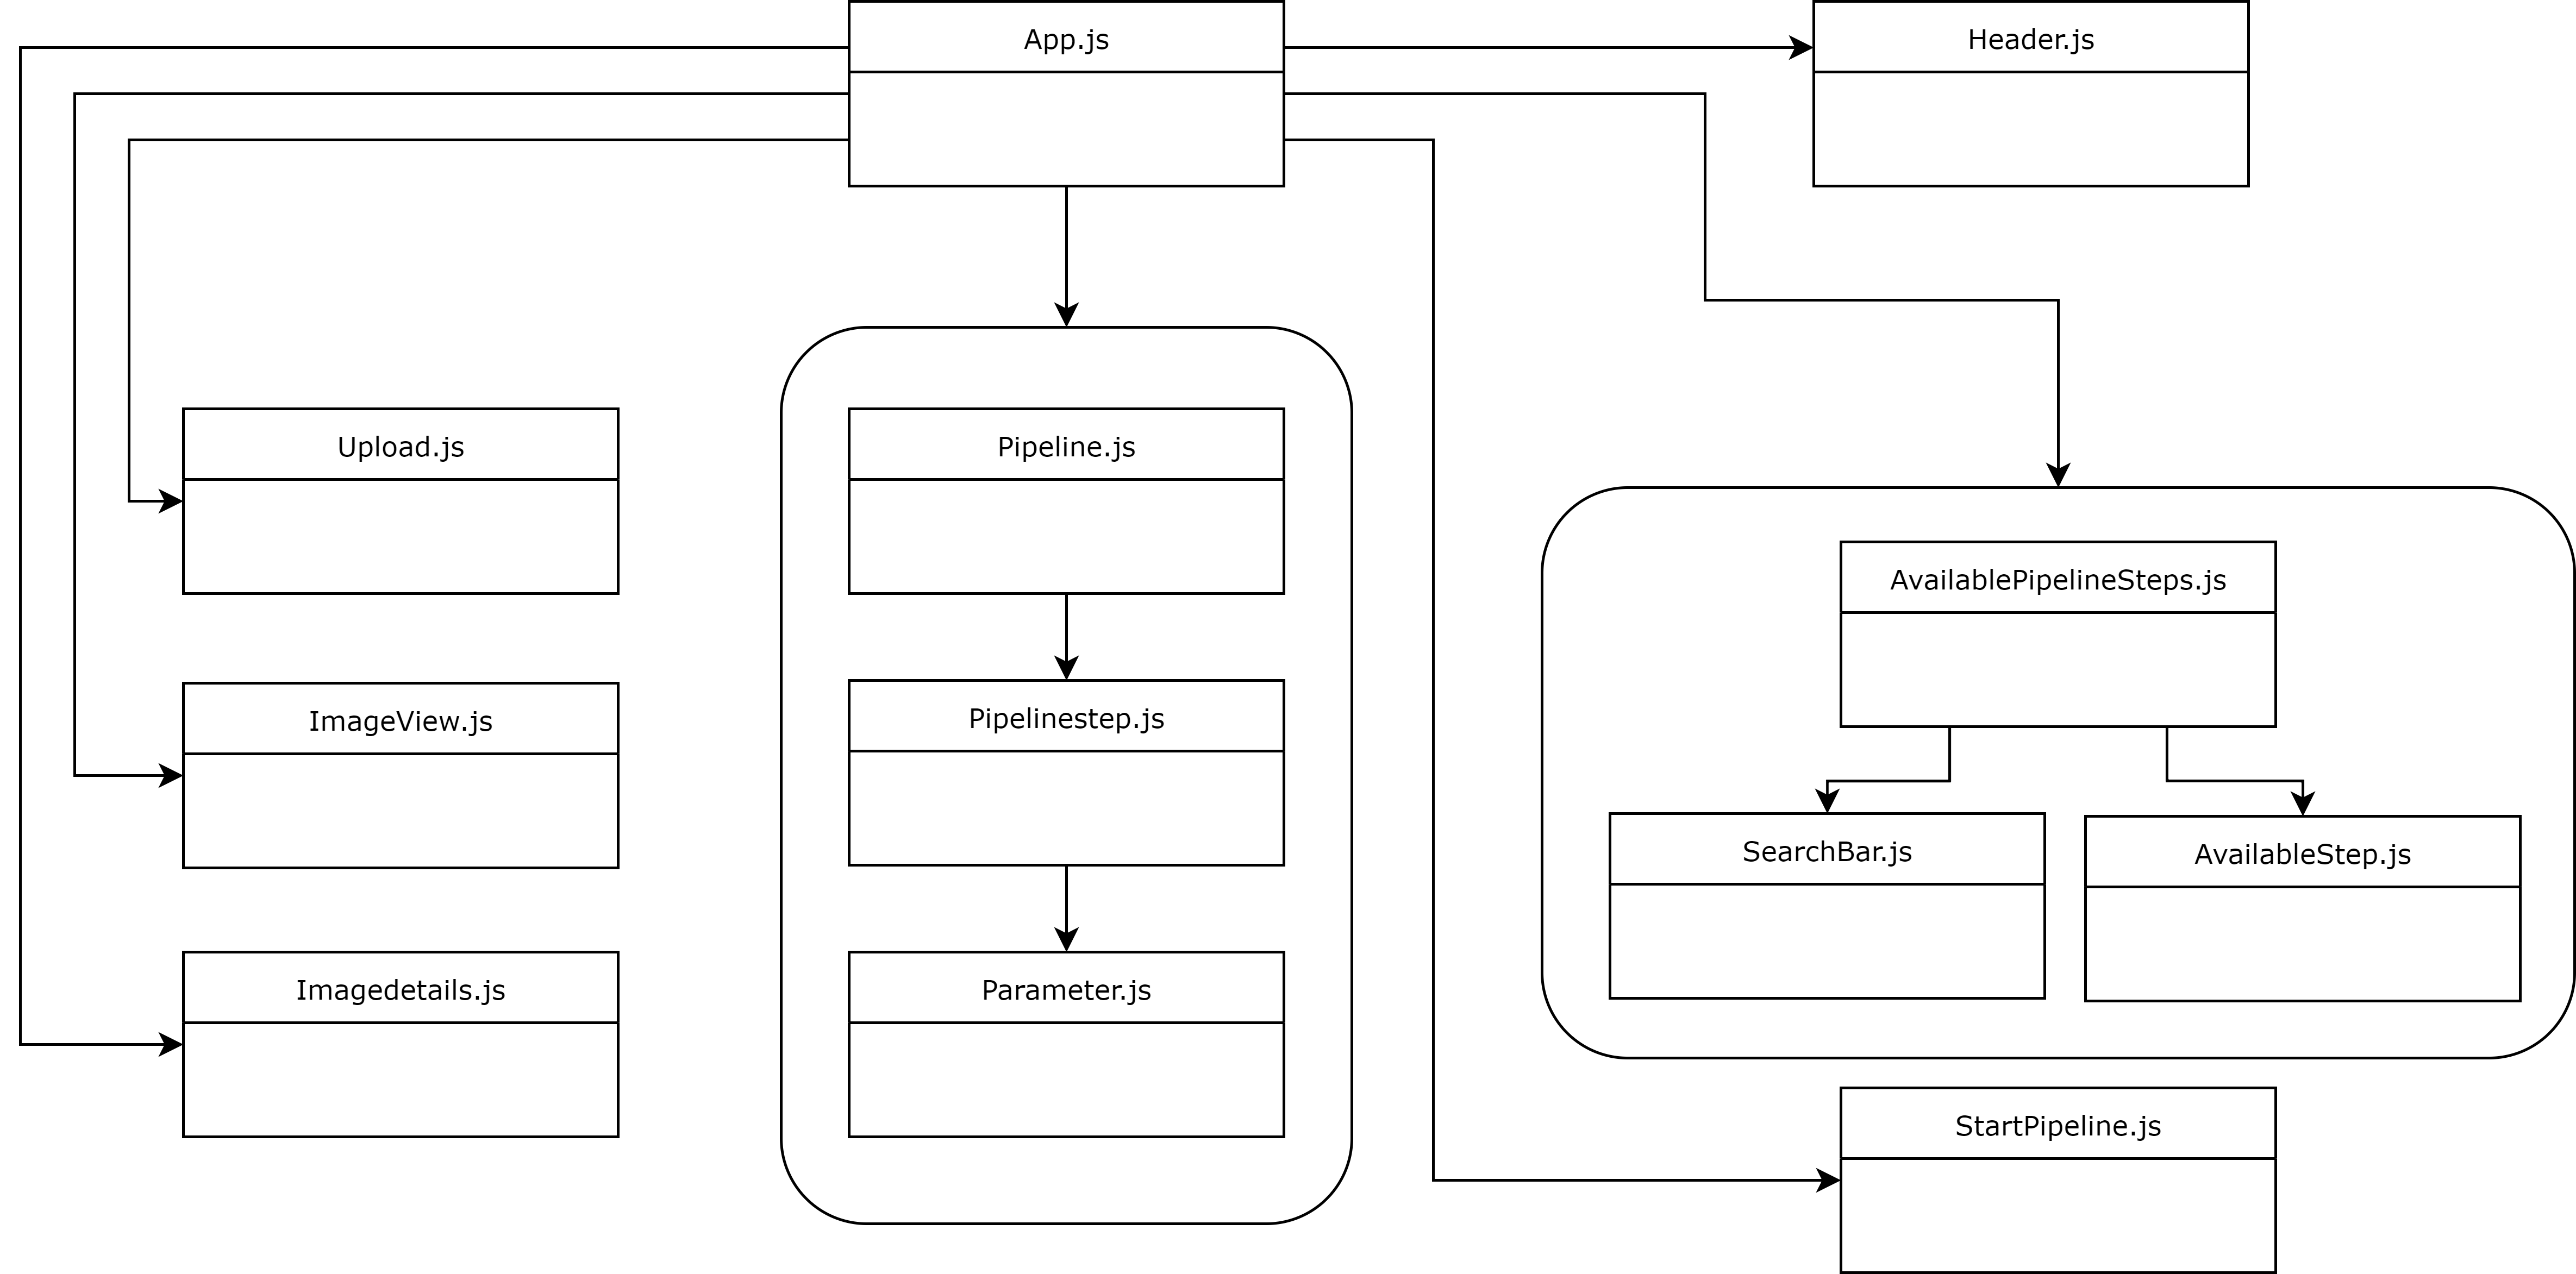
\includegraphics[width=\textwidth]{Bilder/FrontendBDCC.drawio.png}
    \caption{Übersicht der Komponenten im Frontend}
    \label{fig:frontend}
\end{figure*}

\section{Backend: Bildverarbeitung}
Hier steht Backend.

\section{AWS: Amazon Web Services}
\subsection{AWS: Amazon Web Services}
Im Rahmen des Projekts wurde Amazon Web Sevices (AWS) verwendet, um die Anwendung mithilfe einer EC2-Instanz zu verteilen
und die Bilder in einem S3-Bucket zu speichern. Auf den S3-Bucket wird mithilfe, der im Frontend und Backend erstellten Klasse "S3Manager" zugegriffen.

Die Zugriffsrechte wurden in der AWS-Konsole über den Identity und Access Management (IAM) konfiguriert. Dabei wurden feingranulare Rechte an die Benutzer 
vergeben. Dies soll sicherstellen, dass das Frontend und das Backend nur auf den autorisierten Bereich des S3-Buckets zugreifen können. Diese Sicherheitsmaßnahme
soll die anderen Bereiche der Cloud schützen, falls ein Bereich kompromittiert wird.

Durch die Verwendung von AWS und den beiden S3Manager Klassen konnte eine skalierbare Lösung zur Bildspeicherung und -verwaltug bereitgestellt werden.

\section{Fazit und Ausblick}
\section{Fazit und Ausblick}
Das Projekt Computer Vision Pipeline soll den Benutzern eine einfache Schnittstelle zur Verwendung von gängigen Bildverarbeitungsbibliotheken bieten.

Im Fazit lässt sich festhalten, dass das Projektteam trotz der unterschiedlichen Vorkenntnisse erfolgreich zusammengearbeitet hat. Die Einarbeitung in das Frontend-Framework React hat zwar Zeit gekostet, aber letztendlich zu einer ansprechenden und leistungsstarken Benutzeroberfläche geführt. Auch die Implementierung von Tests erwies sich als herausfordernd. Zur Qualitätssicherung des Sytems sind diese aber von großer Bedeutung.

Ein Ausblick auf das Projekt zeigt vieversprechende Möglichkeiten zur Erweiterung der Anwendung. Durch die angelegte Pipelinestruktur im Backend, können mit wenig Aufwand weitere Funktionen eingebaut werden. Da personenbezogene Daten, wie die Bilder, verarbeitet werden, sollte in Betracht gezogen werden die Anwendung um einen Authentifizierung für den Benutzer zu erweitern. Dadurch sollte sichergestellt werden, dass nur der Benutzer auf seine Bilder zugriff hat. Außerdem sollten die Session-Tokens für AWS im Frontend implementiert werden, dass die AWS-Credentials (die Zugangsdaten) temporär an das Frontend übertragen werden. Dies wurde aufgrund der Zeit nicht mehr zu Ende implementiert.5 

\begin{thebibliography}{00}
	\bibitem{scratch} Scratch Programmierung: https://scratch.mit.edu/projects/editor/?tutorial=getStarted
	\bibitem{python} Python: https://www.python.org
	\bibitem{opencv} OpenCV: https://opencv.org
	\bibitem{scikit-image} scikit-image: https://scikit-image.org
	\bibitem{flask} Flask: https://flask.palletsprojects.com/en/2.3.x/
	\bibitem{react} React: https://react.dev
	\bibitem{jest} Jest: https://jestjs.io
	\bibitem{pytest} PyTest: https://docs.pytest.org/en/7.3.x/
\end{thebibliography}
\vspace{12pt}

\end{document}
